\section{Introduction}
\label{sec:intro}
\dan{TODO}
\comment{
\begin{figure}
    \centering
        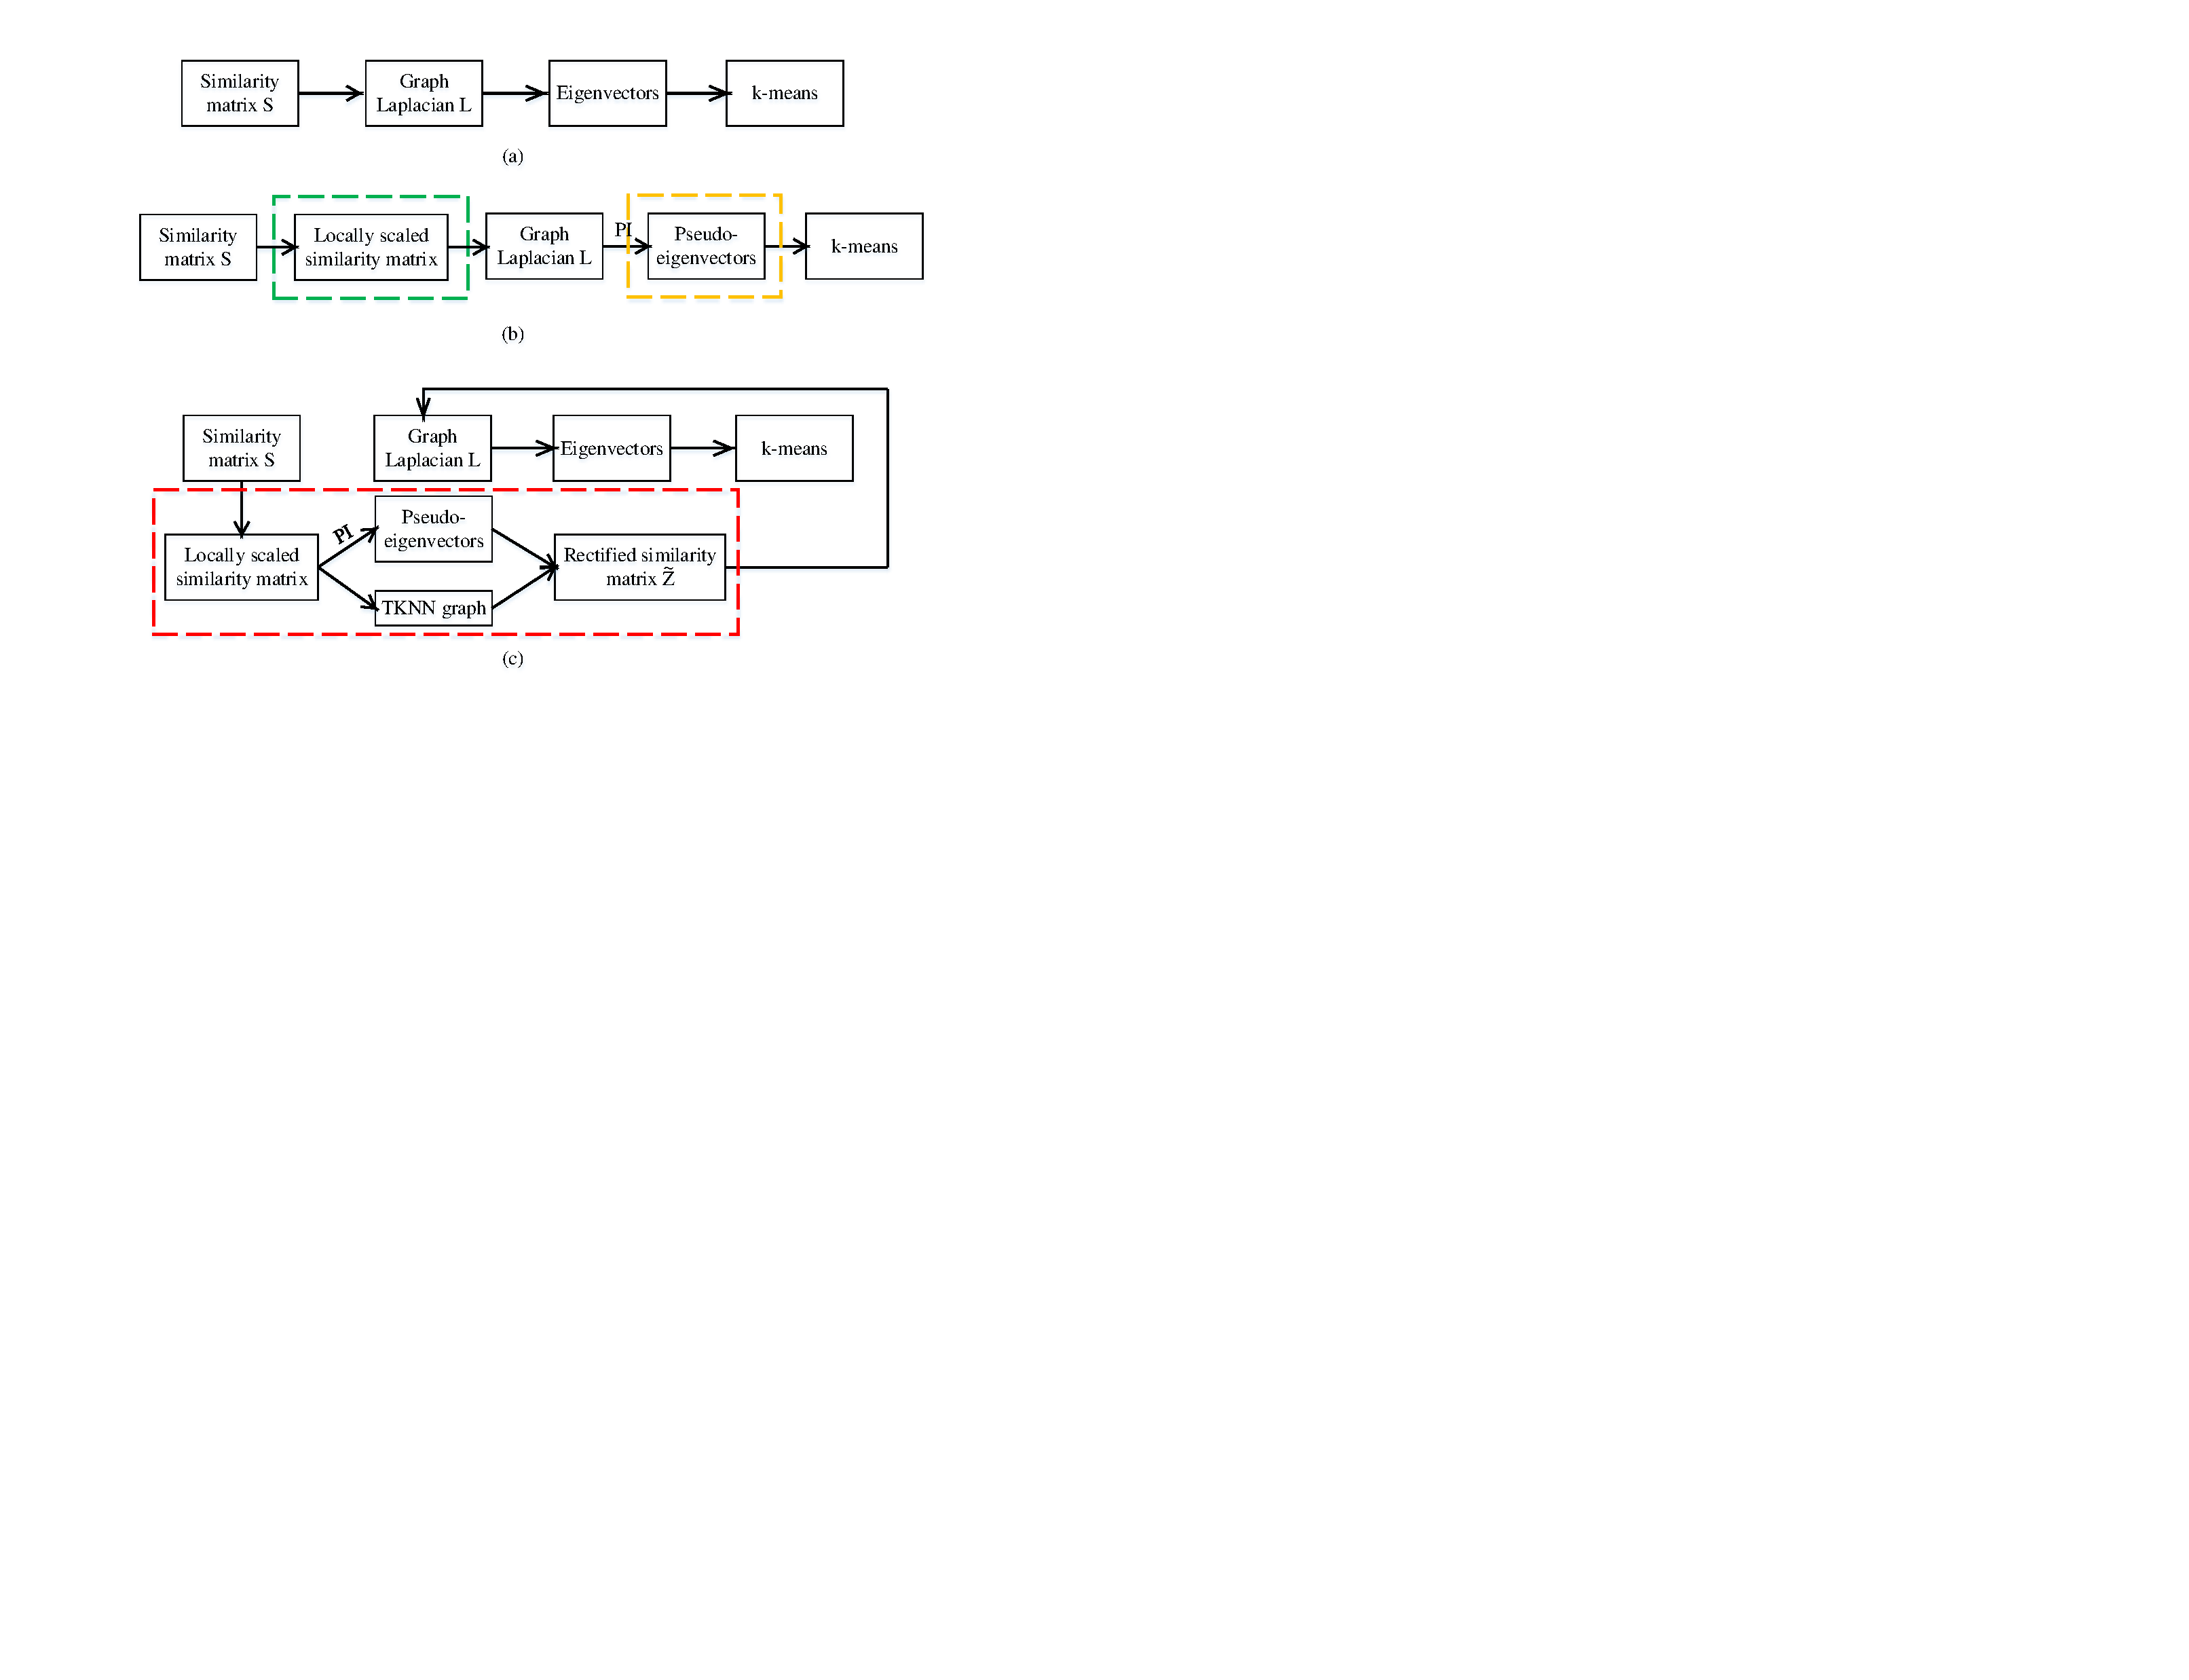
\includegraphics[width = 1.09\linewidth]{flow_graph3.pdf}
        \caption{The key steps of (a) basic spectral clustering; (b) with local scaling and PI; (c) ROSC}
        \label{figure:flow_graph}
\end{figure}
}


Our main contributions are:

\noindent$\bullet$
We proposed a heterogeneous graph convolution algorithm that is capable of capturing edge information.

\noindent$\bullet$
\dan{don't know}

\noindent$\bullet$
We conduct extensive experiments %using synthetic and real datasets 
to evaluate the performance of HINGCN
against $9$ other classification methods. 
Our results show that HINGCN performs very well against the competitors. 
In particular, it is very robust in that it consistently performs well over all the datasets tested. 
Also, it outperforms others by wide margins for datasets that are highly multi-scale. 

The rest of the paper is organized as follows.
%In Section~\ref{sec:preliminary} we give more details of spectral clustering and briefly 
%describe the power iteration method.
Section~\ref{sec:related} mentions related works on heterogeneous graph neural networks, graph embedding and described several semi-supervised classification algorithms.
Section~\ref{sec:algorithm} presents the HINGCN algorithm.
Section~\ref{sec:exp} describes the experiments and presents experimental results.
Finally, Section~\ref{sec:conclusion} concludes the paper.



%\noindent{\small$\bullet$}
%We propose a transitive $K$ nearest neighbor (TKNN) graph.
%In the graph,
%objects in the same cluster but far away in the feature space can be connected
%while objects in different clusters but close to each other can be disconnected.
%
%\noindent{\small$\bullet$}
%We put forward a robust spectral clustering method ROSC on multi-scale data.
%Based on power iteration, ROSC fuses more cluster-separation information in more eigenvectors
%and reduces the redundancy and noise contained.
%%and it integrates the noise reduction with matrix rectification.
%It further applies the TKNN graph to rectify the raw similarity matrix 
%and derives a more effective one,
%leading to a more robust spectral clustering.
%
%\noindent{\small$\bullet$}
%We conduct extensive experiments to
%prove the robustness of ROSC.
%We compare ROSC with state-of-the-art methods on both synthetic and real datasets
%with respect to three clustering measures.
%All the experimental results show that ROSC is indeed a robust spectral clustering method.

\comment{
Recently, in machine learning and computer vision areas, 
%data can be viewed as points drawn from multiple low-dimensional subspaces, with each subspace corresponding to one category or class.
subspace segmentation has been well studied,
which aims to segment (cluster) high-dimensional objects into the low-dimensional subspaces where they are drawn from.
A number of methods have been proposed, such as LRR~\cite{liu2010robust}, LSR~\cite{lu2012robust}, etc.
In these methods, given a set of data vectors $\mathcal{X} = [\bm{x}_1, \bm{x}_2,...,\bm{x}_n]$ (each column is an object) in $\mathbb{R}^d$, 
each object is represented by 
a linear combination of the basis in a dictionary $A = [\bm{a}_1,\bm{a}_2,...\bm{a}_m]$:
\begin{equation}
\nonumber
X = AZ,
\end{equation}
where $Z$ is a coefficient matrix.
Considering the case that data vectors are corrupted by noise, 
a more robust model is thus modified as 
\begin{equation}
\nonumber
X = AZ + E,
\end{equation}
where $E$ is utilized to capture noise.
Subject to the constraint, different optimization objectives on $Z$ (and $E$) are adopted by different methods,
and they desire to derive a low-dimensional mapping $Z$ which can reflect the true subspace structure in the original data.

In this paper, we aim to improve spectral clustering from both effectiveness and efficiency.
Similar to FUSE, we first use power iteration to derive a set of pseudo-eigenvectors 
which inherit all the cluster-separation information in all the eigenvectors.
Then we resort to the subspace segmentation model to purify the pseudo-eigenvectors.

To be continued.
}










